\section{Introduction}


This lab aimed to measure charge distribution over the surface of various shapes in differing scenarios. This objective was accomplished by sampling a point on the object's surface using a proof plane and measuring the voltage using a Faraday Ice Pail. Since voltage is a measure of electric potential difference per unit charge, the changes in voltage were analogous to changes in charge, which is why no conversions between the two were made. Figure 1 depicts how charge density was measured.


\begin{figure}[h]
    \centering
    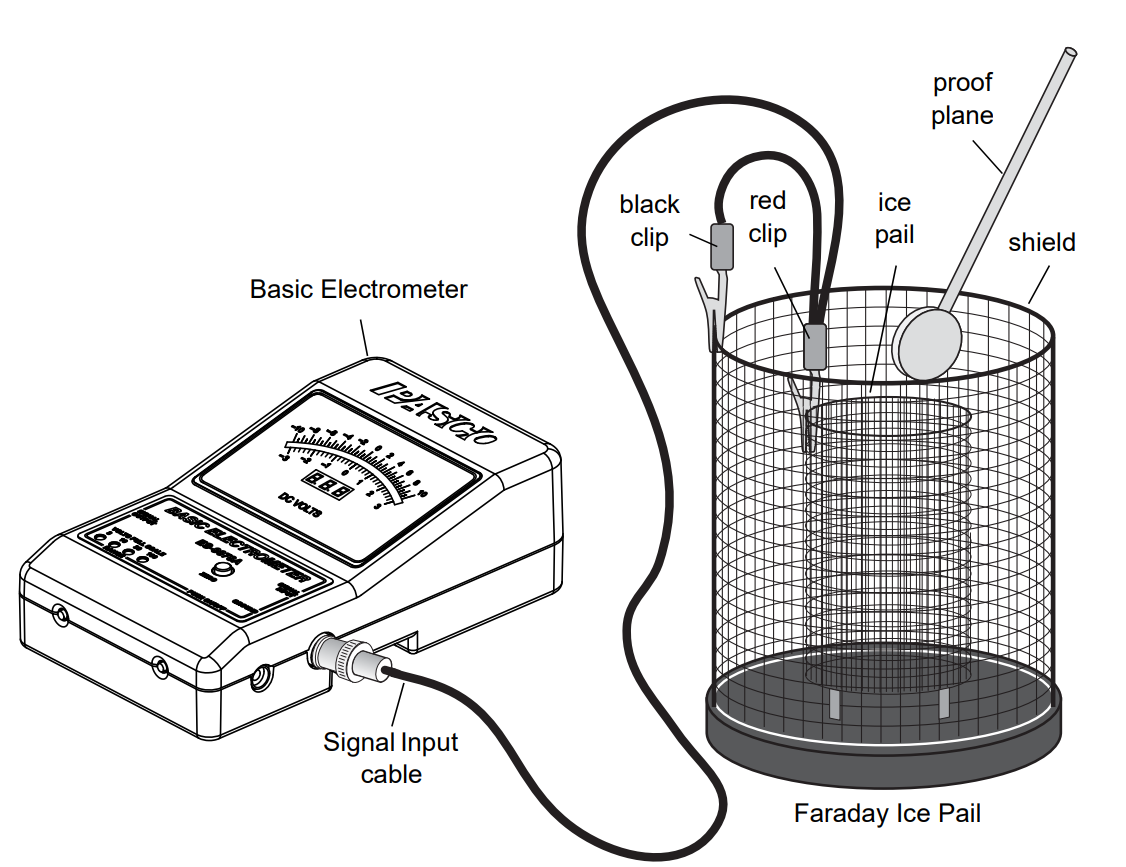
\includegraphics[height=5cm]{photos/equipment.png} 
    \caption{Diagram of the equipment used in the experiments (Basic Electrometer Manual, n.d.)}
    \label{fig:equipment}
\end{figure}

The first experiment utilised two sampling spheres to explore a charged sphere's effect on a grounded sphere. This experiment aimed to observe if a non-uniform charge distribution arose on the sampling sphere due to the attraction of its free-moving electrons towards the positively charged sphere. 

The second and third experiments aimed to analyse the effect a conductor's shape has on its charge distribution. Measurements for experiments 2 and 3 were taken at different points over the surface of a charged conical shape and hollow sphere, respectively. 




\newpage